\chapter{Verification}\label{sec:Verif}

This section will discuss the security properties used by the Read-Only
section of Verified Boot. 
It will also verify these properties using the Hardware and
Software elements that were outlined in Section 2 and Section 3.
All properties are checked using the C Bounded Model Checker (CBMC).
To check some properties, Hardware modules are converted into C using the ILA toolchain.

\section{Vboot Properties}

The properties that will be verified can be separated into 3 categories: array accesses, program flow, and correctness.
The array access property restricts the writeable addresses in memory to valid array boundaries. 
Program flow properties refer to the program's execution path.
Correctness properties refer to facts about the code such that, if things were
designed successfully, certain states should not be reached.
Together these categories of properties should be enough to prove the security claims made by Vboot.

These properties will be specified in Computation Tree Logic (CTL). 
CTL adds temporal distinctions over propositional logic and this allows one to easily describe how a system changes over time.
The boolean connectives in propositional logic are $\lnot$ for NOT, $\land$ for
AND, $\lor$ for OR, and $p \to q$ for $p$ implies $q$.
CTL describes how propositional logic changes through time.
Table~\ref{ctl_syn} describes the CTL syntax.

\begin{table}[!htbp]
    \centering
    \caption{A description of the CTL syntax}\label{ctl_syn}
    \begin{tabular}{ll}
        \toprule Syntax & Description  \\ \bottomrule 
        $Xp$ & $p$ is true in the next state\\ 
        $Fp$ & $p$ is true eventually\\ 
        $Gp$ & $p$ is always true\\ 
    \end{tabular}
\end{table}

\subsection{Memory Access Locations}

Memory accesses in C are very important because C allows for arbitrary addresses to be accessed. 
Addressing arrays before their starting address or after their final address is known as a buffer overrun and it is one of the most common security vulnerabilities. 
Buffer overruns allow a program to write or read to arbitrary memory. 
In Vboot, a buffer overrun could be used to modify the RSA public keys after they have been read in from secure storage, or it could modify the firmware image after it has been verified as secure. 
Such modifications would defeat the security claims of Vboot and for this reason it is important to prevent the accessing of arrays past the array boundaries.

The equation below describes correct array accesses in CTL. 
\begin{equation}
    G(a \to (i > 0 \land i < size(ptr)))
\end{equation}
In this equation $a$ is any array access, $ptr$ is the start of the array and $i$ is the access offset.
This equation states that for every memory access, the index is greater than 0 so it cannot access memory before the array,  and the index is smaller than the size of the array so memory after the array cannot be accessed.

Array indexing is common enough that CBMC provides checking by default.
However, this check on its own is not strong enough to provide array access security for Vboot. 
This is because Vboot uses pointer manipulation in order to access structures and data within the Image. 
Vboot reads the Image from disk as one contiguous binary. 
After the Image has been loaded, the data structures within the Image use size and offset variables to locate more data.
CBMC is not able to automatically detect if this pointer manipulation results in an access outside of the Image.

The following equation defines correct pointer manipulation in Vboot. 
\begin{equation}
    G(\text{offset}(\text{struct}) + \text{size}(\text{struct}) <
    \text{size}(\text{img}) \land \text{offset}(\text{struct}) > 0)
\end{equation}
In this equation $struct$ is the structure being created from a pointer dereference, and $img$ is the image that it is being pointed to.
The equation states that the offset and size of the struct do not go past the edge of the image and that the offset of the struct does is not negative.
We can assume that the offset is not negative because Vboot offsets should only points forward in the Image.

Together these two properties state that array accesses must be in bounds and that structure dereferencing must be in bounds of the image that is being referenced.
As these are the two memory referencing techniques that have the potential for overrun, these properties protect the system against overrun attacks.

\subsection{Program Flow properties}

\begin{figure}
  \centering
  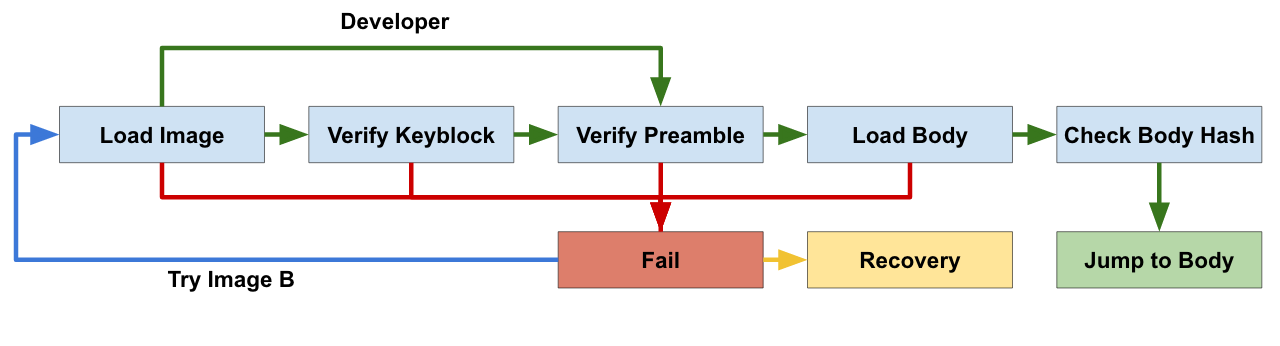
\includegraphics[width=0.6\linewidth]{verification_flow.png}
  \caption[Verified Boot Program Flow]{The logical flow for Vboot.}\label{fig:v_flow}
\end{figure}

There needs to be an ordered constraint on the flow of the program. 
If the program flow is described formally then it will be easy to check that all stages of secure boot were called and in the correct order.
This will catch incorrect programs that skip steps and therefore skip verifying the image, or programs that execute steps out of order and therefore access data that has not been verified yet.
The graph for program flow is shown in Figure~\ref{fig:v_flow}.
When verifying the flow of Vboot it is necessary to note that there are two Images stored in the system, Image A and Image B, and either can be used in the Vboot process. 
It is also necessary to note that Developer mode will skip a step in the verification process, and that this skipped step is a valid part of the Vboot flow.

Let $s_i$ correspond to the ith stage from Figure~\ref{fig:v_flow} and $s_{ai}$ or $s_{bi}$ correspond to that stage for Image A or Image B respectively.

The equation below states that at any time, we must be in at least one of five stages for either image A or image B.
% Must be in a defined state
\begin{equation}
    G(\bigvee\limits_{i = 0}^{4} s_{ai} \lor s_{bi})
\end{equation}

The equation below states the transitions available for Image A.
Each i\textsuperscript{th} stage can transition either to itself or the following stage.
Image A has the ability to fail and transition immediately to the first stage of attesting Image B.

% Image A transitions to next or to B
\begin{equation}
    G(s_{ai} \to s_{ai} \lor s_{ai+1} \lor s_{b0})
\end{equation}

Now we will describe the state transitions for Image B. 
They are similar to Image A but Image B is always tried second and can only transition to the next stage. 
Image B cannot transition back to verifying Image A or it would be possible to have an infinite loop of attesting incorrect images.

% Image B transitions to next
\begin{equation}
    G(s_{bi} \to s_{bi} \lor s_{bi+1})
\end{equation}

The final equation refines the transition for state $s_0$ for Image A and B.
In Figure~\ref{fig:v_flow} we can see that state $s_0$ can transition to $s_1$ but it also has a special transition to $s_2$ that is only valid if Developer Mode is enabled.

% State 0 can skip state 1 if in Developer
\begin{equation}
    G(s_0 \to (s_0 \lor s_{1} \lor (M_D \land s_{2})))
\end{equation}

All together these equations fully describe the program flow graph in Figure~\ref{fig:v_flow}. 
If these hold then steps will not be skipped in the verification process and we can be assured that verification of the image will be attempted in order.

\subsection{Correctness properties}

Correctness properties refer to the code itself and help to determine if it has been written correctly.
For Verified Boot, correctness properties focus on the correct attestation of the image and the guarantee that an incorrect Image cannot be marked as correct and loaded for execution.

The following property states that if the system is not in developer mode and the signature verification fails, then the system will eventually reach the failure state for that image.
It is important that failure and passing is tracked on an image basis because it is possible for Image A to have a bad signature but for Vboot to verify and load a correct Image B.

% Signature is correct when not in Dev mode
\begin{equation} \label{eq:sig_cor}
 \lnot M_d \land \lnot \text{verifySignature(img, rootKey)} \to XF (\text{img.pass} = F)
\end{equation}

The following property states that if the hash of the image data does not match the hash stored in the image, then that specific image will eventually fail.

% Hash is correct always 
\begin{equation} \label{eq:hash_cor}
    \text{hash(img.data)} \neq \text{img.hash} \to XF (\text{img.pass} = F)
\end{equation}

The next property checks against the rollback attack. 
Rollback states that all image versions must be greater than or equal to the last seen image version that is kept in secure storage. 
This property claims that if the image version is lower than what is seen in secure storage, then the image will eventually fail.
Rollback is disabled on Recovery Mode and the property below reflects this fact.

% Version should be greater than previously seen when not in recovery
\begin{equation} \label{eq:rollback}
    \lnot M_r \land (\text{img.version} < \text{prevVersion}) \to XF (\text{img.pass} = F)
\end{equation}

The next property checks that if both images fail, then the Vboot process will fail and the system will eventually reboot into recovery mode.

% If both images fail then boot to recovery 
\begin{equation} \label{eq:both-fail}
    \lnot \text{imgA.pass} \land \lnot \text{imgB.pass} \to XF (\text{pass} = F)
\end{equation}

% TODO: maybe add a Dev wipe property

% TODO: maybe add a hardware return correctly property
% TODO: maybe add that if hash(image) = img.hash -> image = img

In the equations above, img refers to the Image to be verified (either Image A or Image B)  and rootKey is Google's public key that has been loaded out of the GBB.
$M_d$ refers to developer mode being active and $M_r$ refers to recovery mode being active.
Img.version is the Image version number and prevVersion is the last seen version that is stored in the TPM\@.

The contrapositive of these properties will be proved.
The contrapositive of a conditional is the inverse of the condition where the antecedent and consequent are negated.
For example, instead of proving that ``if the hash fails then the image will fail'' it will be proved that ``if the image passes then the hash must have passed''. 
This is easier to check and is logically equivalent.


\section{CBMC}

CBMC is a Bounded Model Checking program for the C language that is released by
Carnegie Mellon. 
A Bounded Model Checker is a tool that performs Formal Verification.
Model checking is a way to exhaustively prove whether a given model meets its
specification.
Model checking typically uses propositional logic or temporal logic. 
At its core, CBMC transforms a C program into binary logic and
then uses a SAT solver to check it against the user's specification. 
The specification is user defined, using an API of C functions defined by the
CBMC library. 

% \begin{figure}
%   \centering
%   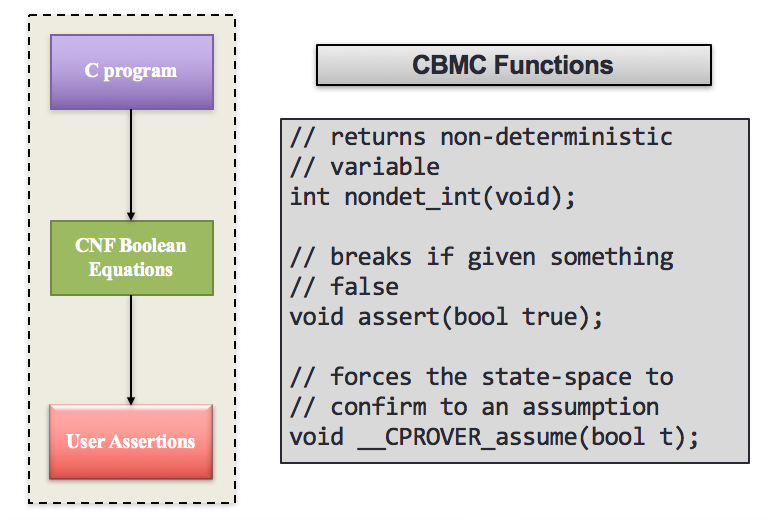
\includegraphics[width=0.7\linewidth]{CBMC_api.png}
%   \caption{The figure on the left describes the transformation that a C
%   program undergoes to be verified. The right describes the CBMC API.}\label{fig:CBMC_api}
% \end{figure}

The CBMC API is very simple.
The list below describes the 3 functions in the CBMC API.

\begin{itemize}
    \item \code{assert(bool e)} -- takes in a boolean expression and throws
        exception if false.
    \item \code{nondet\_int()} -- returns a non-deterministic integer.
    \item \code{assume(bool e)} -- takes in a boolean expression and forces any
        non-deterministic variables to conform.
\end{itemize}

If the \code{assert()} function throws an exception then CBMC will produce a ``counterexample''.
A counterexample lists the program inputs and steps taken that caused the false
assertion.
The \code{nondet\_int()} function is very helpful to model user input to the Vboot process.
Any data that could be modified by the user could feasibly take any
value, and this is represented cleanly by a non-deterministic integer.
CBMC exhaustively checks user assertions against all possible non-deterministic
integer values.

\section{Abstractions}

CBMC was able to be successfully run on portions of the verified boot library and provide information on the satisfiability of various assertions.
Running CBMC on the Read-Only section of Vboot with a full Firmware Image is not possible as the program will consume up to 8GB of RAM on my local machine and then be cancelled.
In order to check properties, abstractions needed to be found such that parts of the Vboot flow could be checked at a single time.

\subsection{Function Over-Abstractions}

The key abstraction used by this thesis is that individual functions are mostly
self contained.
This leads to a natural level abstraction at the function definition.
Each Vboot function returns 0 if successful and an error code if it is not successful.
When a function is abstracted away, it is programmed to return a
non-deterministic value.
If the non-deterministic value is zero (success), then the minimal amount of external changes (if any) should be applied to the larger function.
If the abstracted function returns non-zero (error), then the external changes should be replaced with non-deterministic values.

This method is an over-abstraction of a functions found in the Vboot library.
An over-abstraction contains the full set of states found in the original function, plus additional states that would not be possible.
Because the over-abstraction is a super-set of the original states, any properties that are proved with the over-abstraction will also be proved on every state of the original function.
Therefore any properties proved with abstracted functions will also hold if the real functions were left in place.

\subsection{Loop Removal}

Another helpful abstraction is to remove long loops that are present in Verified
Boot.
CMBC performs loop unrolling before it performs any model checking. 
In a program with long loops, the unrolling adds unnecessary complexity and
state to the model and it increases checking time dramatically.
All of Vboots long loops are comparing or copying arrays.
An array compare can be abstracted into a single non-deterministic read on both
arrays.
An array copy can be abstracted into a single non-deterministic write on the
array.
Because the index into the array is non-deterministic in both cases, CBMC will
still perform verification on every acceptable index and find possible
counterexamples.
This abstraction was taken from an earlier thesis that also performed Formal
Verification~\cite{elane}. 

\subsection{Memory Allocation}

The final abstraction is the creation of a simple memory allocation function so
CBMC will handle pointer manipulation correctly.
Vboot data structures contain offsets to other data structures, not full
pointers. 
Vboot uses offsets because the data structures are loaded from disk and there is
no guarantee that the data will be loaded into a specific address.
(There is however, a guarantee that the data will be loaded contiguously)
The following code shows the simple pointer arithmetic needed for offsets.

\begin{equation} \label{eq:ptr}
\begin{split}
    \code{uint32\_t offset = \&data - \&image;} \\
    \code{void *data\_ptr = \&image + offset;} 
\end{split}
\end{equation}

However, CBMC will not perform pointer arithmetic unless the original pointer
was set to a specific value.
A small memory management function was created to assign pointer values to data
structures so CBMC would perform the correct arithmetic.
In this abstraction memory addresses start at 0x0 and increase as needed.
Memory is never reclaimed.
The idea for this abstraction originated from the work done in modeling memory
by Franjo Ivancic\cite{eff-model-check}.

\section{Verifying Vboot with CBMC}

This section describes the verification tests on Vboot using CBMC\@.
Each subsection begins with a diagram showing the functional call graph of what section of code is being verified.
The diagrams are color-coordinated as followed.
The blue functions are fully software functions that are implemented in the Vboot Library.
The yellow functions connect to the Flash firmware on a real platform, but have been abstracted to return either non-deterministic data for Read-Write information, or hardcoded data for Read-Only information.
The red functions connect to the TPM on a real platform, and are verified on the
ILA TPM for this report.
The purple functions connect to Vboot's software RSA library. 
The green functions connect to the ILA SHA model. 

For each function being verified, the connecting functions are replaced with
abstractions.
These abstractions all follow the idea of an ``over-abstracted'' function.
The abstracted functions can be seen in my Code Repo or the code included in the
Appendix.

Finally, there will be a table describing the results of each CBMC run.
CMBC uses an implementation of a SAT solver known as the MiniSat solver\cite{minisat}.
This solver outputs unSAT if the assertions hold and SAT if they do not. 
The ``steps'' column is the number of C lines that were stepped through to reach the proof conclusion.
The ``VCC'' column is the number of user assertions that were being verified.

\subsection{Google's Assertions}

Google has already created a Unit Test Framework for the Verified Boot process.
This framework tests various properties of each function.
Like most Unit Testing Frameworks, the functions are not tested in conjunction
with the rest of the system.
The framework given also stubs out any calls to Hardware, meaning that it 
will not catch any errors across the Hardware Software boundary.
Finally, the framework only checks for the input conditions provided. 
Each function tested has roughly five to fifteen input conditions that are
checked, which is not exhaustive.

Luckily, the framework that Google uses also relies on assertions.
This project was able to hook Google's Unit Test assertions into CBMC
assertions, so Google specific properties can be verified for free along with 
the larger security properties. 

\subsection{LoadFirmware}

\begin{figure}[!htbp]
  \centering
  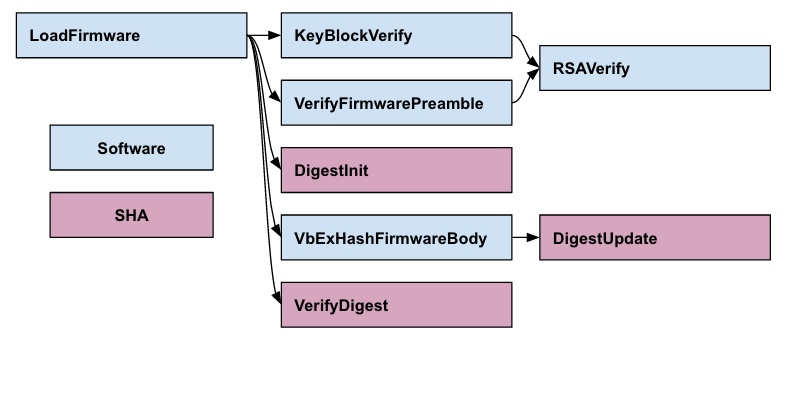
\includegraphics[width=0.6\linewidth]{loadfw.png}
  \caption[LoadFirmware Call Graph]{The call graph of functions for LoadFirmware}\label{fig:loadfw}
\end{figure}

LoadFirmware is the highest level function that drives Vboot's Firmware Image
verification process.
LoadFirmware is responsible for verifying the Keyblock, Preamble, and Image.
When LoadFirmware returns, it will have set the pass or fail statuses of both Firmware Images, and control will pass to a working Image.

The CBMC test results for this function can be seen in Table~\ref{ldfw_results}. 
Below is an itemized list of what each test is verifying.

\begin{itemize}
 \item  Google Assertions -- this test replaces Google's assertions with CBMC assertions and checks that none of them are violated under any inputs
 \item  rollback test -- tests that under no input conditions will LoadFirmware choose a firmware image with a lower version number (see Property~\ref{eq:rollback}).
 \item  rollback/rec  -- this test is supposed to find a counter-example. It tests for rollback conditions without realizing that rollback is allowed under recovery. 
 \item  hash failure -- tests that it is impossible to verify an image as correct  if hashing the Firmware body (the VbExHashFirmwareBody function) returns an error (see Property~\ref{eq:hash_cor}).
 \item  RSA failure -- tests that is impossible to verify an image as correct if verifying either the Keyblock or Preamble returns an error (see Property~\ref{eq:sig_cor}).
 \item  Array accesses -- check for all possibilities of array bounds errors.
\end{itemize}

\begin{table}[!htbp]
    \centering
    \caption{CBMC tests on the LoadFirmware function}\label{ldfw_results}
    \begin{tabular}{llllll}
        \toprule
        test name & steps & VCCs  & time (s) & sat/unsat  \\ \bottomrule
        Google Assertions & 6460 & 34 & 67.02 & unsat \\
        rollback     & 4125 & 1 & 4.79 & unsat \\
        rollback/rec & 4123 & 1 & 4.68 & sat \\
        Hash Failure & 4182 & 2 & 4.45 & unsat \\
        RSA  Failure & 4180 & 2 & 4.45 & unsat \\
        Array Accesses & 4130 & 22 & 4.51 & unsat \\
    \end{tabular}
\end{table}

We can see from these tests that CBMC is working successfully and in a reasonable time.
The counter example of the ``rollback/rec'' test quickly pointed the user to the counterexample where the Recovery Mode allowed rollback.
These results also show that Formal Verification tools are a possibility for checking the assertions that already exist in Google's testing framework.

\subsection{VbSelectFirmware}

\begin{figure}[!htbp]
  \centering
  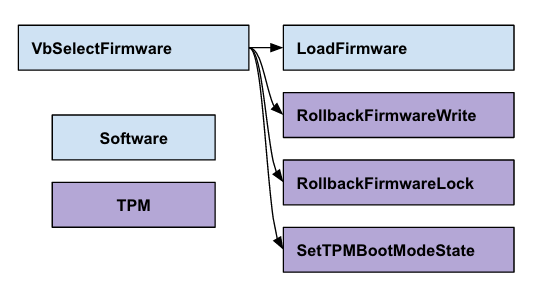
\includegraphics[width=0.4\linewidth]{vb_sel_fw.png}
  \caption[VbSelectFirmware Call Graph]{The call graph of functions for VbSelectFirmware}\label{fig:vbselfw}
\end{figure}

The VbSelectFirmware function is the wrapper around LoadFirmware.
It is responsible for loading flags in from secure storage and for accessing the TPM\@.
VbSelectFirmware is also responsible for locking the TPM's firmware version before control passes to the firmware image and updating the version if a newer image has been loaded.
This function's final responsibility is to load TPM's PCR0 with the hash of the boot flags.

\begin{itemize}
 \item  TPM locking -- tests that it is not possible for the function to return success if it is unable to lock the TPM
 \item  LoadFirmware -- tests that it is not possible for control to pass to an Image if it is not selected by LoadFirmware
 \item  Array accesses -- check for all possibilities of array bounds errors.
\end{itemize}

\begin{table}[!htbp]
    \centering
    \caption{CBMC tests on function VbSelectFirmware}\label{sfw_results}
    \begin{tabular}{llllll}
        \toprule
        test name & steps & VCCs & time (s) & sat/unsat  \\ \bottomrule
        TPM locking & 5269 & 6 & 0.07 & unsat \\
        LoadFirmware & 5264 & 2 &  0.07 & unsat \\
        Array Accesses & 5257 & 0 & 0 &  unsat \\
    \end{tabular}
\end{table}

\section{TPM Properties}

\begin{figure}[!htbp]
  \centering
  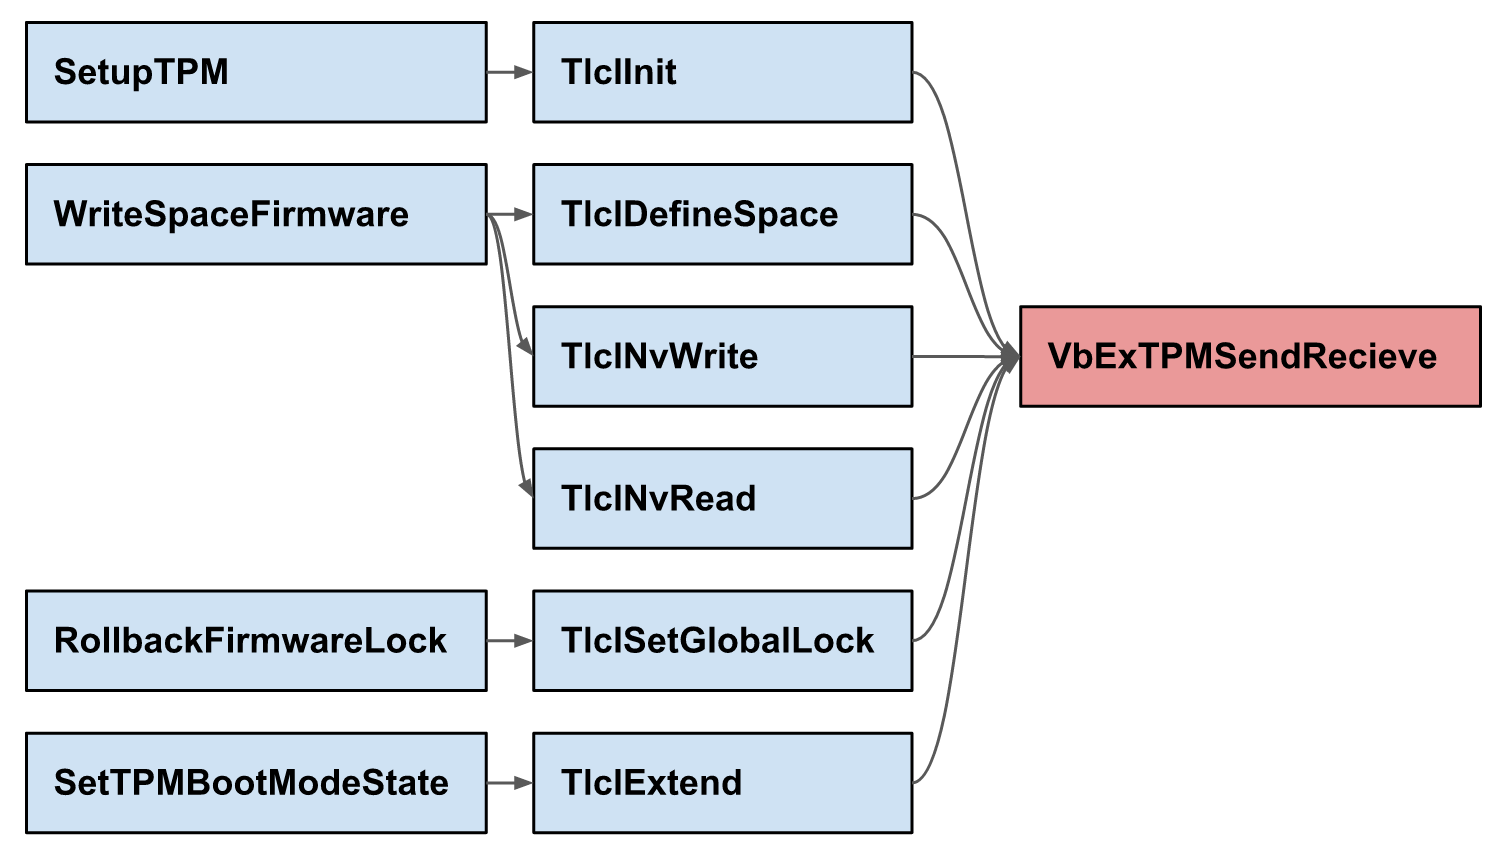
\includegraphics[width=0.6\linewidth]{tpm_call_graph}
  \caption[TPM Call Graph]{This shows the Vboot call graph for the TPM functionality}\label{fig:tpm_call_graph}
\end{figure}

The Read-Only Firmware is responsible for setting up the TPM and protecting its
sections against the rest of the system that will eventually be loaded.
TPM's responsibilities from Chrome are to securely store the boot state and the
version state.
TPM's storage of the version state allows Vboot to claim that it protects against 
an attacker loading an older, less secure image from Google (Rollback attack).
TPM's storage of the boot state allows Vboot to claim protection against an attacker loading a Google Developer image onto a non-developer machine.

In earlier sections we checked software properties by abstracting the TPM to a simple storage array. 
This allowed us to check the larger rollback and protection properties, although we were assuming that the TPM Firmware functions were working correctly.
Now, we will be using the TPM's Firmware and an abstraction of Hardware to verify correctness of the TPM's Firmware functions.

The bulk of properties that will be checked are Correctness and Liveness properties. 

% Rollback Attack

\subsection{ILA for Hardware}   

\subsection{TPM Properties}   

%TODO get graph of Vboots TPM functions
Some properties are possible to prove using Hardware and Firmware separately.
The first run is showing that each TPM function will only return true if it receives the ``success'' back from the TPM\@.
Once we have this property we can also prove that the TPM will only return the ``success'' value if its operations are completed successfully. 
Combining these two properties can give us an idea of correctness for the system.

However, there are some properties that are much easier to prove with the 
Hardware and Firmware together.
In the third run we have the property that the firmware will always read every available byte from the TPM command fifo.
This property is important to show the Firmware is correct and it relies on interactions between Hardware and Firmware.
The fourth run checks that each function will always return. 
This is important for liveness, because if the Firmware is stuck polling a register forever then the system will not boot.

%TODO: Get TPM CBMC table up and running here

\subsection{Verifying TPM with ILA}   

In order to check the TPM, the Vboot firmware had to use the TPM registers and
command flow described in Section~\ref{tpm_cmd_regs}.
This was accomplished by creating an abstraction of the TPM using the ILA framework.
This abstraction described the TPM registers and command functionality in a way that could be verified by CMBC\@.
The TPM abstraction contains only the subset of the TPM functionality required by Vboot, which was outlined in Section~\ref{sec:TPM}.

The TPM ILA code can be seen in the appendix.
The file \code{TPM\_template.py} is the ILA template.
The file \code{TPM\_simulator.py} is a python simulator of the TPM registers that
were  used for verification.
The simulator and the template are a formal description of the TPM's registers and command behavior that were outlined previous in Section~\ref{tpm_cmd_regs}. 
